\documentclass[a4paper,12pt]{scrreprt}
\usepackage[T1]{fontenc}
\usepackage[utf8]{inputenc}
\usepackage[ngerman]{babel}
\usepackage[table]{xcolor}% http://ctan.org/pkg/xcolor
\usepackage{tabu}
\usepackage{graphicx}
\usepackage{lmodern}
\begin{document}


%\titlehead{Kopf} %Optionale Kopfzeile
\author{Daniel Dimitrijevic \and Thomas Traxler} %Zwei Autoren
\title{ XVSM Benchmark } %Titel/Thema
\subject{VSDB} %Fach
\subtitle{ Mozartspaces } %Genaueres Thema, Optional
\date{\today} %Datum
\publishers{5AHITT} %Klasse

\maketitle
\tableofcontents


\chapter{Aufgabenstellung}
	Realisieren Sie mithilfe der bereitgestellten Implementierung (Autofabrik) das definierte 	Koordinationsproblem möglichst effizient mit der XVSM Implementierung "MozartSpaces". Setzen Sie dabei Notifications [2Pkt] und Transaktionen [2Pkt] sinnvoll ein (bei Bedarf auch Aspekte [+2ExtraPkt]).\\\\
	Die in der Implementierung bereitgestellten Teile des Produktionsroboters sollen in den Space geschrieben werden [2Pkt]. Anschließend sollen die Einzelteile zu Autos 
	zusammengebaut, getestet und schließlich ebenfalls in den Space ausgeliefert werden 
	[2Pkt]. Weitere Anhaltspunkte entnehmen Sie bitte der beigelegten Anforderungsanalyse.\\\\
	Überlegen Sie sich eine entsprechende Containerstruktur [2Pkt]. Jedes Einzelteil und jedes zusammengebaute Auto soll durch ein eigenes Objekt im Space repräsentiert werden (und nicht etwa in einer Liste, die als Ganzes in den Space geschrieben wird). Jeder Roboter wird dabei als eigener Prozess gestartet. Diese Prozesse können als einfache Konsolenapplikationen implementiert werden, bei denen die ID als Argument übergeben wird. Die Kommunikation zwischen den Robotern darf nur über den gemeinsamen Space erfolgen, der vor dem Starten der Roboter gestartet und evtl. initialisiert werden muss. Die Anzeigetafel erhält alle Informationen nur über den Space [2Pkt]. Prozesse für die Roboter sollen jederzeit dynamisch gestartet oder geschlossen werden können, ohne dass die Funktionalität beeinträchtigt wird.\\\\
	Stellen Sie zu guter Letzt in einem Benchmark Ihre XVSM-Implementierung der RMIImplementierung gegenüber und überprüfen Sie auf Performance, Skalierbarkeit und 
	Aufbau des Source-Codes [4Pkt]. Beachten Sie dabei mögliche Patterns. Dokumentieren 
	Sie ausführlich all Ihre Codeänderungen. Vergessen Sie dabei nicht auf die Beschreibung der neu verwendeten Technologien.
	
\chapter{XVSM}
	XVSM (eXtensible Virtual Shared Memory). XVSM ist eine Middleware Technology
	die Daten in “Container” speichert und für andere Peers teilt. Dieser Weg bringt einige Vorteile wie die Daten werden auf mehreren verschiedenen Computern verteilt, damit wird die Ausfallwahrscheinlichkeit der Daten reduziert.
\chapter{Arbeitsaufteilung}
	\tabulinesep = 4pt
	\begin{tabu}  {|[2pt]X[2.5,c] |[1pt] X[4,c] |[1pt]X[1.3,c]|[1pt]X[c]|[2pt]}
		\tabucline[2pt]{-}
		Name & Arbeitssegment & Time Estimated & Time Spent\\\tabucline[2pt]{-}
		
		Traxler \and Dimitrijevic& Protokoll & 0.5h & 0.5h\\\tabucline[1pt]{-}
		Traxler & Container Struktur& 1h & 1h\\\tabucline[1pt]{-}
		Traxler & CarFactory to XVSM& 2h & 2.5h \\\tabucline[1pt]{-}
		Dimitrijevic & Roboter to XVSM & 2h & 3.5h \\\tabucline[1pt]{-}
		Dimitrijevic & Testing & 1h & 1h \\\tabucline[1pt]{-}
		Dimitrijevic \and Traxler & Benchmarking & 1h & 1h \\\tabucline[2pt]{-}
		Gesamt && 7.5h & 9.5h \\\tabucline[2pt]{-}
	\end{tabu}	

\chapter{UML}

\begin{figure}
\centering
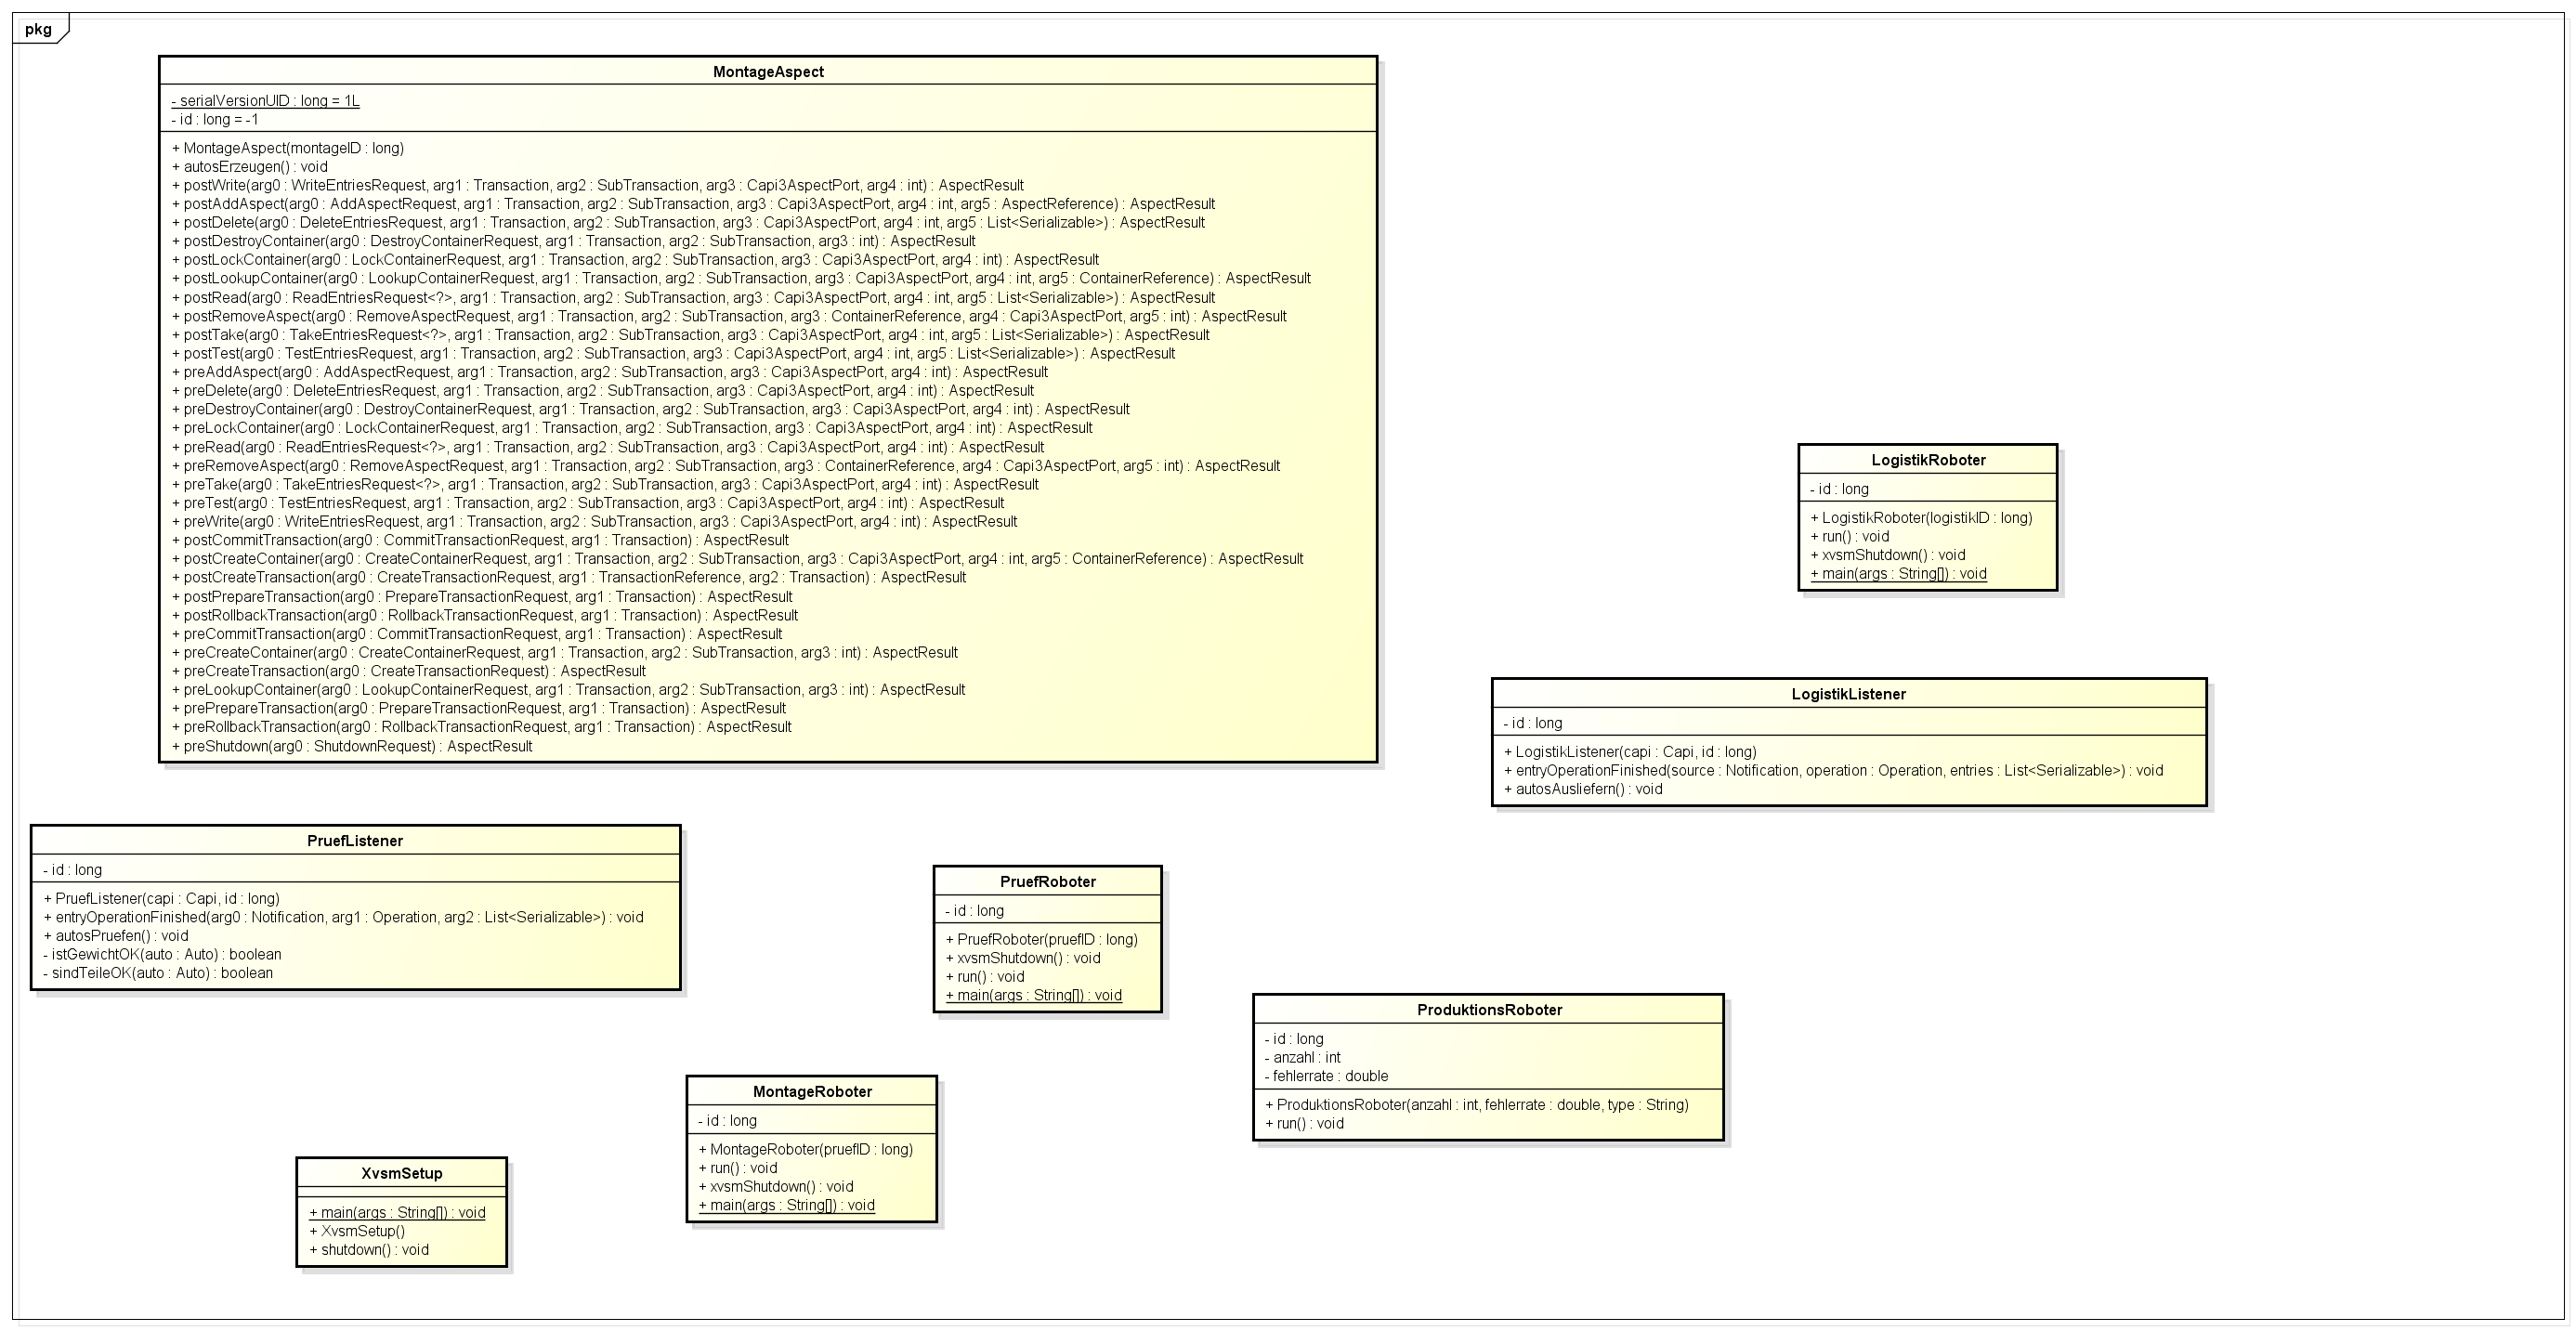
\includegraphics[width=0.7\linewidth]{./XVSM_UML_1}
\caption{}
\label{fig:XVSM_UML_1}
\end{figure}
\begin{figure}
\centering
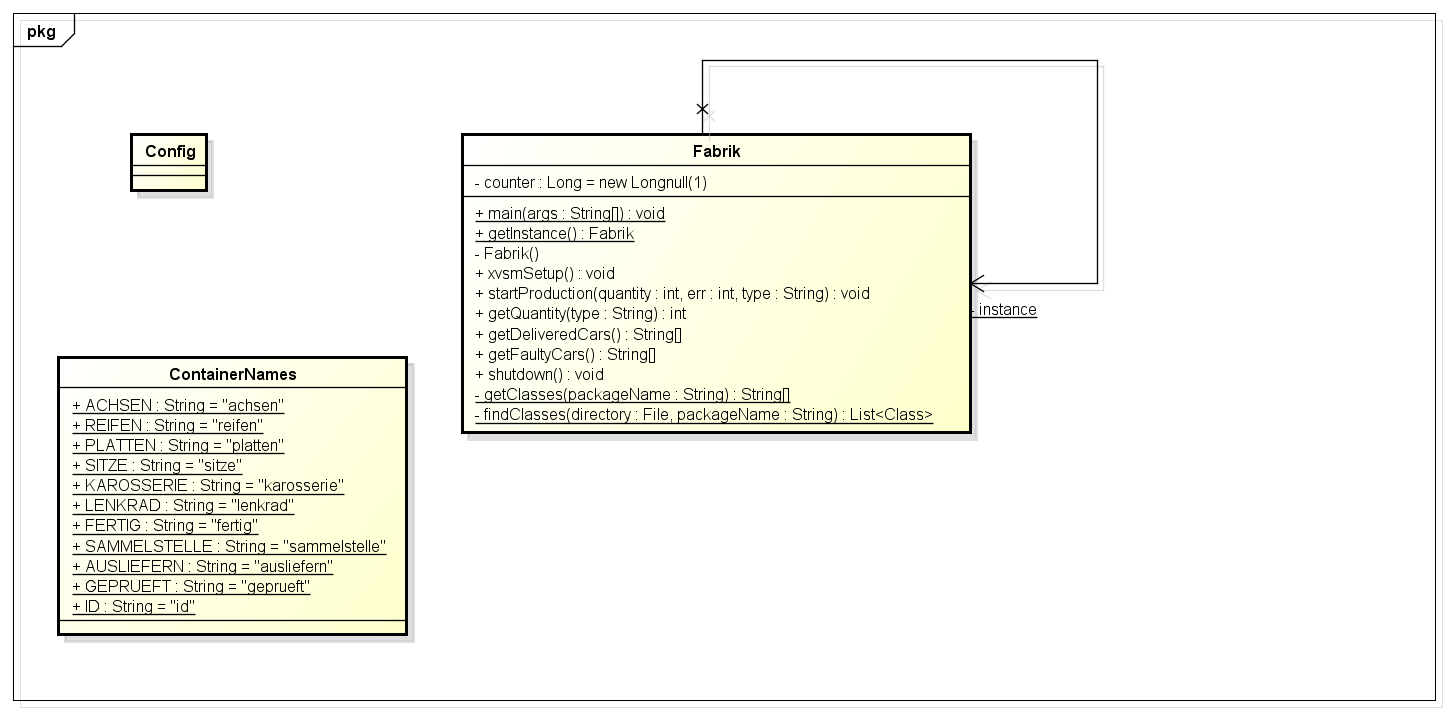
\includegraphics[width=0.7\linewidth]{./XVSM_UML_2}
\caption{}
\label{fig:XVSM_UML_2}
\end{figure}

\chapter{Arbeitsdurchführung}

	Ein gro"ses Problem das wir vorfanden war, dass das Mozartspaces System bei jeder Verbindung neue Threads erzeugt welche weiter wartend waren nachdme die Verbindung beendet wurde so sammelte sich eine Unzahl an TCP-Connection Threads an wenn das System zuviele Anfragen bekommen hat.
	
\chapter{Benchmarks}
	\section{Unter RMI}
\begin{figure}[h]
\centering
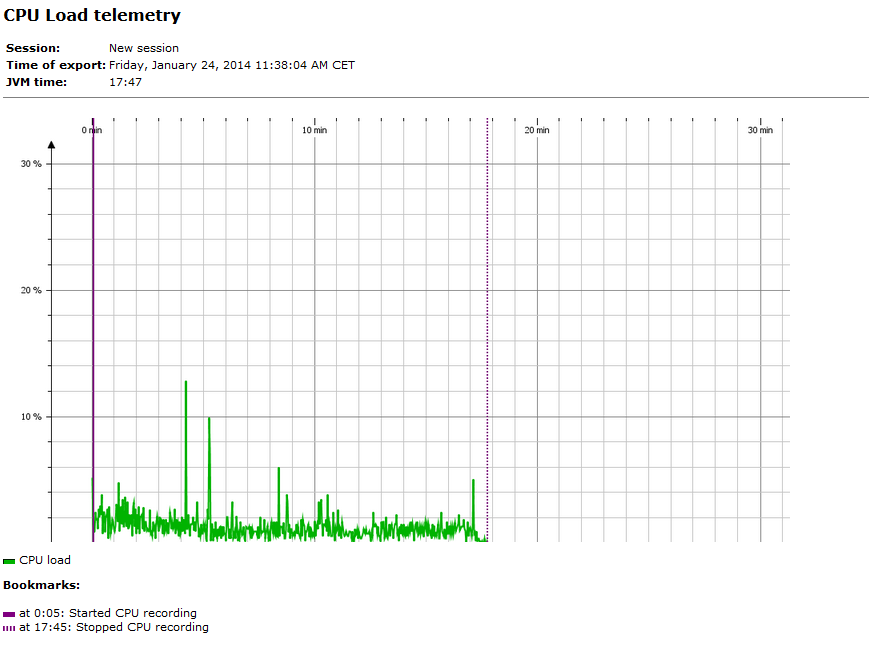
\includegraphics[width=0.6\linewidth]{./CPU_Load_Telemetry_RMI}
\caption{}
\label{fig:CPU_Load_Telemetry_RMI}
\end{figure}
\begin{figure}[h]
\centering
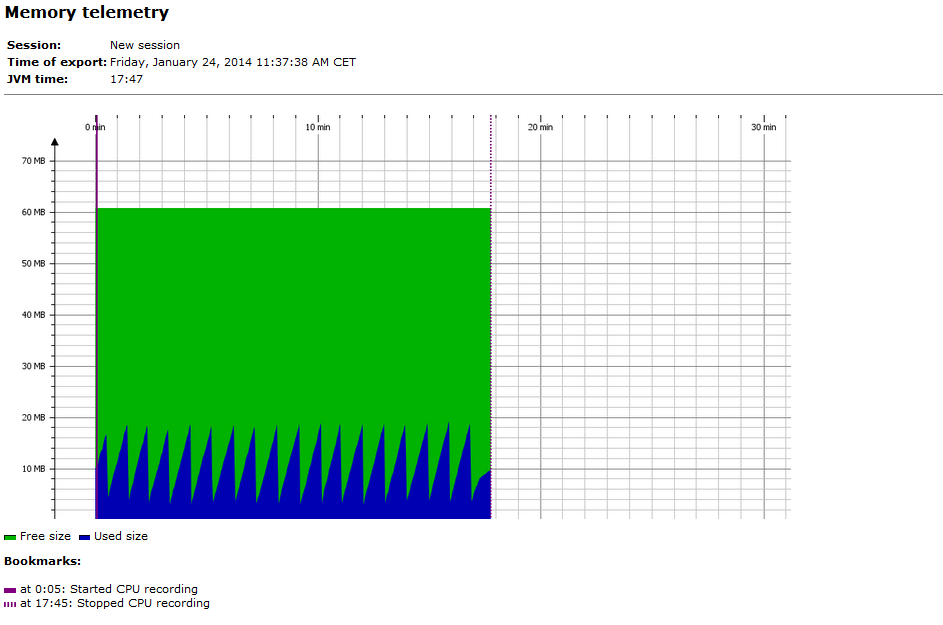
\includegraphics[width=0.6\linewidth]{./Memory_RMI}
\caption{}
\label{fig:Memory_RMI}
\end{figure}
\begin{figure}[h]
\centering
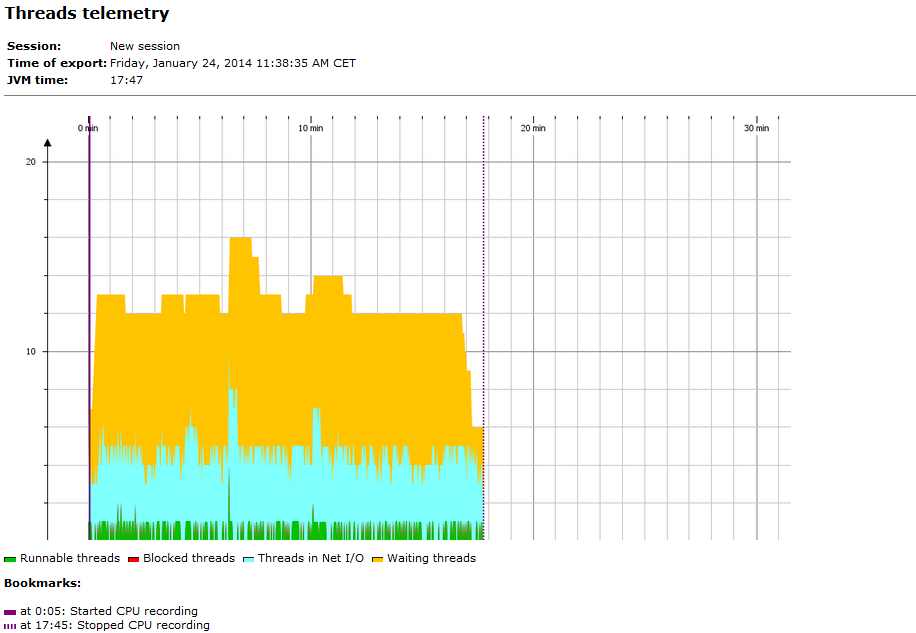
\includegraphics[width=0.6\linewidth]{./Thread_RMI}
\caption{}
\label{fig:Thread_RMI}
\end{figure}



\pagebreak

\pagebreak
\section{XVSM}
\begin{figure}[h]
\centering
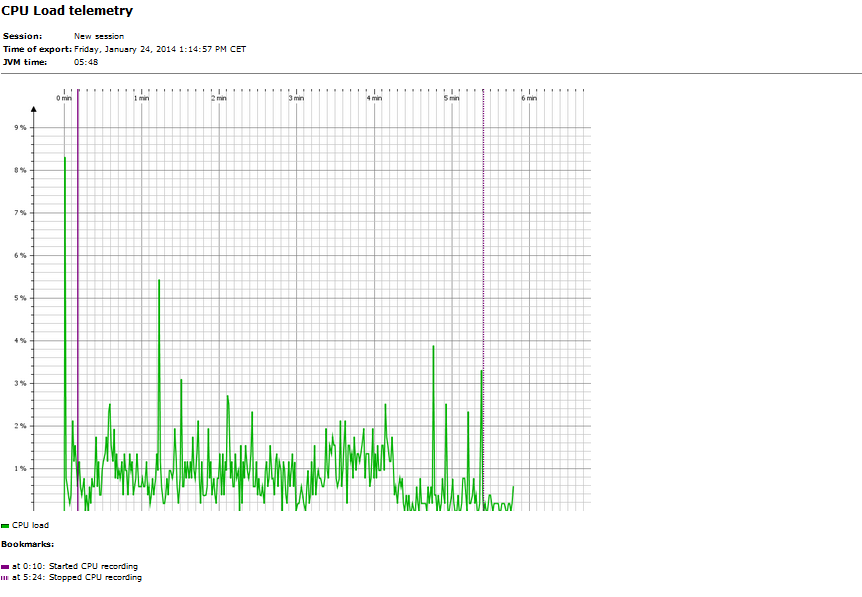
\includegraphics[width=0.6\linewidth]{./CPU_XVSM}
\caption{}
\label{fig:CPU_XVSM}
\end{figure}
\begin{figure}[h]
\centering
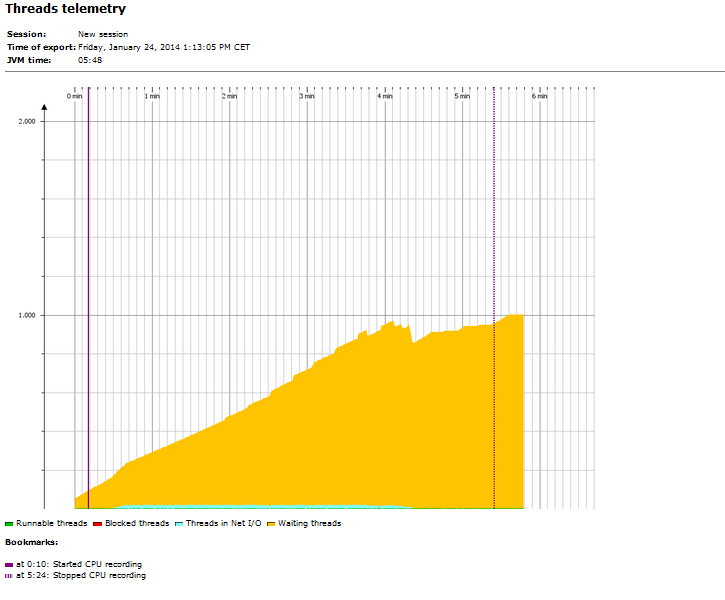
\includegraphics[width=0.6\linewidth]{./Thread_XVSM}
\caption{}
\label{fig:Thread_XVSM}
\end{figure}







\end{document}